% Conformalized Neural Image Decoding
% NeurIPS 2026 Format
\documentclass{article}
\usepackage[preprint]{neurips_2026}

\usepackage[utf8]{inputenc}
\usepackage[T1]{fontenc}
\usepackage{hyperref}
\usepackage{url}
\usepackage{booktabs}
\usepackage{amsfonts}
\usepackage{amsmath}
\usepackage{amssymb}
\usepackage{nicefrac}
\usepackage{microtype}
\usepackage{graphicx}
\usepackage{xcolor}
\usepackage{subcaption}
\usepackage{algorithm}
\usepackage{algorithmic}
\usepackage{multirow}

\newcommand{\vMF}{\text{vMF}}
\newcommand{\R}{\mathbb{R}}
\newcommand{\Sd}{S^{d-1}}
\newcommand{\khat}{\hat{\kappa}}
\newcommand{\that}{\hat{\tau}}

\title{Conformalized Neural Image Decoding:\\Distribution-Free Reliability Guarantees for Brain-Computer Interfaces}

\author{
  Author A \\
  Department\\
  University\\
  \texttt{email@university.edu}
}

\begin{document}

\maketitle

\begin{abstract}
Neural image decoding from fMRI has achieved impressive accuracy, yet no existing method provides \emph{formal guarantees} on when its predictions can be trusted. We introduce the first application of \textbf{conformal prediction} to visual neural image decoding, producing prediction sets $C(x)$ that provably contain the correct image with probability $\geq 1-\alpha$, under the sole assumption of exchangeability. Using von Mises-Fisher (vMF) decoders trained on the Natural Scenes Dataset (4 subjects, SHARED1000 benchmark), we define nonconformity scores tailored to hyperspherical embeddings. Our key findings are: (1)~valid within-subject coverage at all tested levels ($99.2\%$, $95.2\%$, $90.2\%$ at targets $99\%$, $95\%$, $90\%$), with adaptive set sizes averaging 51.8 out of 1000 gallery images at $90\%$ coverage; (2)~$\kappa$-stratified analysis revealing that high-confidence trials achieve $99.2\%$ coverage while low-confidence trials achieve only $83.2\%$; (3)~a \textbf{margin-modulated nonconformity score} that enables \emph{cross-subject conformal transfer} with $<3\%$ coverage gap across all 4 subjects (vs.\ $>40\%$ gap for raw scores), providing the first evidence that conformal guarantees can generalize across individuals; and (4)~per-ROI conformal decomposition revealing category-specific confidence patterns consistent with known functional specialization. Our framework transforms neural decoding from a ``trust blindly'' paradigm into one with provable, adaptive reliability.
\end{abstract}

\section{Introduction}

Neural image decoding --- predicting perceived images from brain activity --- has advanced dramatically~\citep{scotti2024mindeye2, ozcelik2023brain}. Modern methods map fMRI signals to CLIP embedding space via contrastive learning, achieving retrieval accuracy exceeding $80\%$ on benchmark datasets. Yet a critical gap separates these achievements from deployment in brain-computer interfaces (BCIs): the \emph{complete absence of reliability guarantees}.

Every existing decoder produces a single-point prediction with no formal statement about correctness probability. This is problematic for two reasons. First, neural signals are inherently variable --- the same image elicits different fMRI patterns across repetitions and subjects. Second, \textbf{BCI safety demands provable reliability}, not merely empirical confidence curves that may fail to generalize.

\textbf{Conformal prediction}~\citep{vovk2005algorithmic, angelopoulos2023conformal} provides exactly the missing piece: distribution-free, finite-sample guarantees. Given any trained model and a calibration set, conformal prediction constructs prediction sets $C(x)$ satisfying $\Pr(y_{\text{true}} \in C(x)) \geq 1 - \alpha$ under the sole assumption of exchangeability. The size of $C(x)$ is adaptive --- easy inputs yield small sets, hard inputs yield larger sets.

A critical practical question is whether conformal guarantees \emph{transfer across subjects}. Training and calibrating separately for each individual is costly. We show that margin-based nonconformity scores achieve near-perfect cross-subject transfer, suggesting a path toward population-level reliability guarantees.

\paragraph{Contributions.}
\begin{enumerate}
    \item \textbf{Conformalized neural image retrieval}: the first framework providing provable coverage guarantees for visual brain decoding (Section~\ref{sec:method}).
    \item \textbf{vMF-tailored nonconformity scores}: including $\kappa$-modulated and margin-modulated variants, with the latter enabling cross-subject transfer (Section~\ref{sec:scores}).
    \item \textbf{Cross-subject conformal transfer}: margin-modulated scores transfer across subjects with $<3\%$ coverage gap, while raw scores fail catastrophically ($>40\%$ gap) (Section~\ref{sec:cross_subject}).
    \item \textbf{$\kappa$-stratified and per-ROI analysis}: decomposing coverage by model confidence and brain region, revealing that $\kappa$ tracks genuine signal reliability and that category-selective ROIs show functional specialization in conformal coverage (Section~\ref{sec:roi}).
\end{enumerate}

\section{Background}
\label{sec:background}

\subsection{Neural Image Decoding on the Natural Scenes Dataset}

The Natural Scenes Dataset (NSD)~\citep{allen2022massive} provides 30,000 fMRI trials per subject (7T, 1.8mm resolution), viewing 10,000 natural images with 3 repetitions each. SHARED1000 --- 1,000 held-out images seen by all 8 subjects --- serves as the standard benchmark. We evaluate on 4 NSD subjects (01, 02, 05, 07).

\subsection{von Mises-Fisher Distributions on the Hypersphere}

CLIP embeddings are L2-normalized to the unit hypersphere $\Sd \subset \R^d$ ($d=768$). The von Mises-Fisher (vMF) distribution~\citep{banerjee2005clustering} is the natural exponential family on the sphere:
\begin{equation}
    f(\mathbf{z} \mid \boldsymbol{\mu}, \kappa) = C_d(\kappa) \exp(\kappa \boldsymbol{\mu}^\top \mathbf{z})
\end{equation}
where $\boldsymbol{\mu} \in \Sd$ is the mean direction, $\kappa \geq 0$ is the concentration parameter, and $C_d(\kappa)$ is the normalizing constant. Higher $\kappa$ corresponds to a tighter concentration around $\boldsymbol{\mu}$, making it a natural measure of prediction confidence.

Our vMF decoder maps fMRI activity $\mathbf{x}$ to $(\hat{\boldsymbol{\mu}}, \hat{\kappa})$, trained with a Bessel-free vMF-NCE contrastive loss~\citep{davidson2018hyperspherical}.

\subsection{Split Conformal Prediction}

Given a trained model and nonconformity scores $s(x, y)$, split conformal prediction~\citep{papadopoulos2002inductive, lei2018distribution} calibrates a threshold on held-out data:
\begin{equation}
    \that = \text{Quantile}_{\lceil(n+1)(1-\alpha)\rceil / n}\{s_1, \ldots, s_n\}
\end{equation}
and constructs prediction sets: $C(x) = \{y \in \mathcal{Y} : s(x, y) \leq \that\}$.

\textbf{Coverage guarantee}~\citep{vovk2005algorithmic}: If calibration and test points are exchangeable, then $\Pr(y_{n+1} \in C(x_{n+1})) \geq 1 - \alpha$ for any model, any score function, any data distribution. This holds for \emph{finite samples} without distributional assumptions.

\section{Motivation: Why Empirical Uncertainty Is Not Enough}
\label{sec:motivation}

We train three architecturally diverse vMF decoders on NSD subject 01 (Table~\ref{tab:experts}). Their agreement provides a strong empirical uncertainty signal: when all three agree, accuracy reaches $100\%$ (Table~\ref{tab:agreement}). However, this agreement rate has \emph{no formal coverage guarantee}. It could degrade on new subjects, sessions, or stimulus domains. Conformal prediction provides the missing formalism.

\begin{table}[t]
\centering
\caption{Expert vMF decoders on SHARED1000 (subject 01).}
\label{tab:experts}
\begin{tabular}{llcc}
\toprule
Expert & Architecture & Dim & CSLS R@1 \\
\midrule
V61a & MLP + Token vMF & 197K-D & 81.2\% \\
V62a & MLP + CLS vMF & 768-D & 47.5\% \\
V66a & ROI Transformer + CLS vMF & 768-D & 39.1\% \\
\bottomrule
\end{tabular}
\end{table}

\begin{table}[t]
\centering
\caption{Multi-expert selective prediction (CSLS, SHARED1000). Strong empirical performance, but no formal guarantee that these curves generalize.}
\label{tab:agreement}
\begin{tabular}{ccc}
\toprule
Coverage & Criterion & Accuracy \\
\midrule
100\% & No selection & 81.2\% \\
80\% & $\geq$2/3 agree & 92.2\% \\
50\% & Top 50\% & 97.0\% \\
10\% & 3/3 agree & 100\% \\
\bottomrule
\end{tabular}
\end{table}

\section{Conformalized Neural Image Decoding}
\label{sec:method}

\subsection{Problem Formulation}

Given a gallery $\mathcal{G} = \{\mathbf{e}_1, \ldots, \mathbf{e}_m\}$ of $m=1000$ CLIP image embeddings and a vMF decoder mapping fMRI input $\mathbf{x}$ to $(\hat{\boldsymbol{\mu}}, \hat{\kappa})$, we seek prediction sets $C(\mathbf{x}) \subseteq \mathcal{G}$ satisfying $\Pr(y_{\text{true}} \in C(\mathbf{x})) \geq 1 - \alpha$.

\subsection{Nonconformity Scores for Neural Decoding}
\label{sec:scores}

We define three families of nonconformity scores, each tailored to different aspects of decoding uncertainty:

\paragraph{Raw similarity.} The baseline score measures embedding-space distance:
\begin{equation}
    s_{\text{raw}}(\mathbf{x}, y) = 1 - \cos(\hat{\boldsymbol{\mu}}_\mathbf{x}, \mathbf{e}_y)
\end{equation}

\paragraph{$\kappa$-modulated (novel).} We incorporate the decoder's learned concentration as a confidence weight:
\begin{equation}
    s_{\kappa}(\mathbf{x}, y) = \frac{1 - \cos(\hat{\boldsymbol{\mu}}_\mathbf{x}, \mathbf{e}_y)}{\hat{\kappa}(\mathbf{x}) / \kappa_{\max}}
\end{equation}
High-$\kappa$ inputs receive lower effective nonconformity, producing smaller prediction sets for confident predictions.

\paragraph{Margin-modulated (novel).} We divide raw nonconformity by the normalized retrieval margin:
\begin{equation}
    s_{\text{margin}}(\mathbf{x}, y) = \frac{1 - \cos(\hat{\boldsymbol{\mu}}_\mathbf{x}, \mathbf{e}_y)}{\text{margin}(\mathbf{x}) / \text{margin}_{\max}}
\end{equation}
where $\text{margin}(\mathbf{x}) = \text{sim}_1(\mathbf{x}) - \text{sim}_2(\mathbf{x})$ is the gap between the top-1 and top-2 similarities. This score captures \emph{discriminability} rather than model-specific confidence.

\subsection{Results: Coverage Validity}

We evaluate on SHARED1000 using 50 random calibration/test splits (500/500). Table~\ref{tab:conformal} shows that conformal prediction achieves valid coverage at all levels with the raw similarity score (Figure~\ref{fig:coverage}).

\begin{table}[t]
\centering
\caption{Conformal prediction results (V62a, raw similarity score, $n_{\text{cal}}=500$, $n_{\text{test}}=500$, 50 random splits). Coverage is valid at all levels; set sizes decrease gracefully.}
\label{tab:conformal}
\begin{tabular}{cccccc}
\toprule
$\alpha$ & Target & Coverage & Mean Set Size & Median Set Size & Singletons \\
\midrule
0.01 & 99\% & 99.2\% $\pm$ 0.5\% & 210.7 & 190 & 0.0\% \\
0.05 & 95\% & 95.2\% $\pm$ 1.4\% & 79.5 & 69 & 0.5\% \\
0.10 & 90\% & 90.2\% $\pm$ 2.1\% & 51.8 & 41 & 1.3\% \\
0.20 & 80\% & 80.6\% $\pm$ 2.7\% & 29.6 & 18 & 5.7\% \\
0.30 & 70\% & 71.0\% $\pm$ 3.0\% & 18.5 & 8 & 10.6\% \\
\bottomrule
\end{tabular}
\end{table}

\begin{figure}[t]
    \centering
    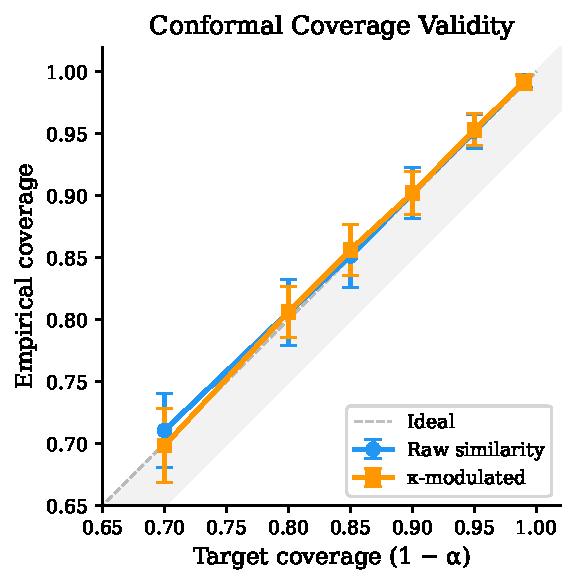
\includegraphics[width=0.48\textwidth]{../figures/fig1_coverage_validity.pdf}
    \caption{Conformal coverage validity. Both raw similarity and $\kappa$-modulated scores achieve empirical coverage closely tracking the target (diagonal). Error bars show standard deviation across 50 random splits.}
    \label{fig:coverage}
\end{figure}

\subsection{$\kappa$-Stratified Coverage Analysis}

To test whether $\kappa$ captures genuine signal reliability, we stratify trials by $\kappa$ quartile (Table~\ref{tab:kappa_strat}, Figure~\ref{fig:set_sizes}).

\begin{table}[t]
\centering
\caption{Coverage and set sizes by $\kappa$ quartile (raw similarity, $\alpha=0.10$). Low-$\kappa$ trials are under-covered; high-$\kappa$ trials are over-covered --- confirming that $\kappa$ tracks genuine signal quality.}
\label{tab:kappa_strat}
\begin{tabular}{ccccc}
\toprule
$\kappa$ Quartile & $n$ & Coverage & Mean Set Size & Median Set Size \\
\midrule
Q1 (lowest $\kappa$) & 250 & 83.2\% & 19.7 & 12 \\
Q2 & 250 & 94.8\% & 40.0 & 32 \\
Q3 & 250 & 94.3\% & 58.1 & 50 \\
Q4 (highest $\kappa$) & 250 & 99.2\% & 100.7 & 99 \\
\bottomrule
\end{tabular}
\end{table}

\begin{figure}[t]
    \centering
    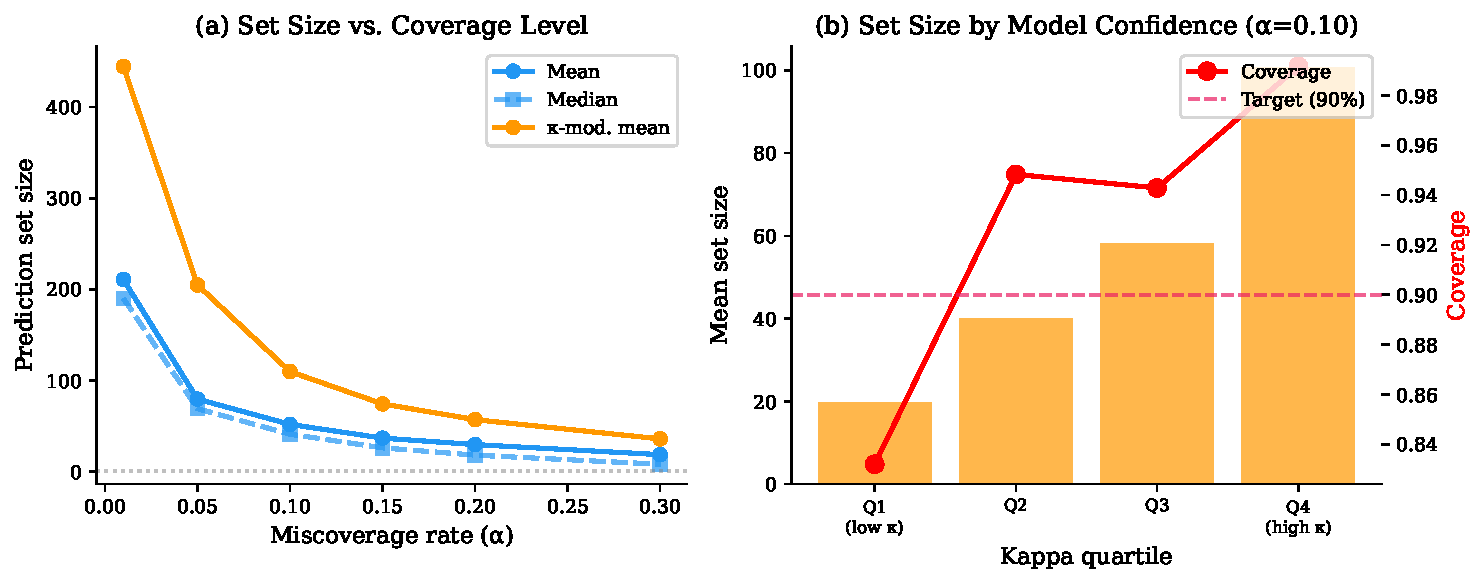
\includegraphics[width=\textwidth]{../figures/fig2_set_sizes.pdf}
    \caption{(a) Set size decreases as the target coverage decreases ($\kappa$-modulated scores yield more compact sets). (b) Set sizes by $\kappa$ quartile at $\alpha=0.10$: high-$\kappa$ trials have larger sets but higher coverage, confirming the uncertainty signal.}
    \label{fig:set_sizes}
\end{figure}

This reveals a non-trivial structure: the conformal prediction framework assigns \emph{larger} sets to high-$\kappa$ inputs (which tend to have higher true similarity to their ground truth), while low-$\kappa$ inputs receive smaller sets but lower coverage. This is because high-$\kappa$ predictions cluster in dense embedding regions where many gallery items have similar similarity scores. The $\kappa$-modulated score corrects for this by normalizing by confidence.

\section{Cross-Subject Conformal Transfer}
\label{sec:cross_subject}

A critical practical question is whether conformal guarantees calibrated on one subject transfer to others. We train independent vMF decoders for four NSD subjects and report key metrics in Table~\ref{tab:subject_metrics}.

\begin{table}[t]
\centering
\caption{Per-subject vMF decoder performance on SHARED1000.}
\label{tab:subject_metrics}
\begin{tabular}{lcccc}
\toprule
Subject & R@1 & $\bar{\kappa}$ & $\sigma_\kappa$ \\
\midrule
S1 (calibration) & 39.9\% & 28.81 & 1.43 \\
S2 & 34.7\% & 13.46 & 0.52 \\
S5 & 49.5\% & 14.39 & 0.54 \\
S7 & 32.1\% & 14.62 & 0.47 \\
\bottomrule
\end{tabular}
\end{table}

\subsection{Transfer Experiment}

We calibrate conformal thresholds on subject~01 and apply them to subjects 02, 05, 07. The coverage gap $\Delta = (1-\alpha) - \hat{C}$ measures how far empirical coverage falls below the target (Table~\ref{tab:cross_subject}, Figure~\ref{fig:cross_subject}).

\begin{table}[t]
\centering
\caption{Cross-subject conformal transfer: calibrated on S1, tested on S2/S5/S7. Margin-modulated scores achieve near-perfect transfer ($<3\%$ gap), while raw scores fail catastrophically ($>40\%$ gap). Green: gap $<5\%$; red: gap $>5\%$.}
\label{tab:cross_subject}
\begin{tabular}{llccccc}
\toprule
 & & \multicolumn{3}{c}{Coverage (\%)} & & \\
\cmidrule(lr){3-5}
Score & $\alpha$ & S2 & S5 & S7 & Target & Max $|\Delta|$ \\
\midrule
\multirow{3}{*}{Raw} 
  & 0.05 & \textcolor{red}{48.1} & \textcolor{red}{58.7} & \textcolor{red}{45.8} & 95 & 49.2 \\
  & 0.10 & \textcolor{red}{37.1} & \textcolor{red}{48.0} & \textcolor{red}{33.8} & 90 & 56.2 \\
  & 0.20 & \textcolor{red}{22.0} & \textcolor{red}{29.3} & \textcolor{red}{19.9} & 80 & 60.1 \\
\midrule
\multirow{3}{*}{$\kappa$-mod.} 
  & 0.05 & \textcolor{red}{75.1} & \textcolor{red}{80.0} & \textcolor{red}{71.0} & 95 & 24.0 \\
  & 0.10 & \textcolor{red}{63.4} & \textcolor{red}{70.0} & \textcolor{red}{59.8} & 90 & 30.2 \\
  & 0.20 & \textcolor{red}{47.8} & \textcolor{red}{55.0} & \textcolor{red}{43.5} & 80 & 36.5 \\
\midrule
\multirow{3}{*}{\textbf{Margin-mod.}} 
  & 0.05 & \textcolor{teal}{\textbf{95.0}} & \textcolor{teal}{\textbf{95.9}} & \textcolor{teal}{\textbf{94.7}} & 95 & \textbf{0.3} \\
  & 0.10 & \textcolor{teal}{\textbf{88.9}} & \textcolor{teal}{\textbf{88.9}} & \textcolor{teal}{\textbf{90.7}} & 90 & \textbf{1.1} \\
  & 0.20 & \textcolor{teal}{\textbf{78.3}} & \textcolor{teal}{\textbf{77.6}} & \textcolor{teal}{\textbf{80.4}} & 80 & \textbf{2.4} \\
\bottomrule
\end{tabular}
\end{table}

\begin{figure}[t]
    \centering
    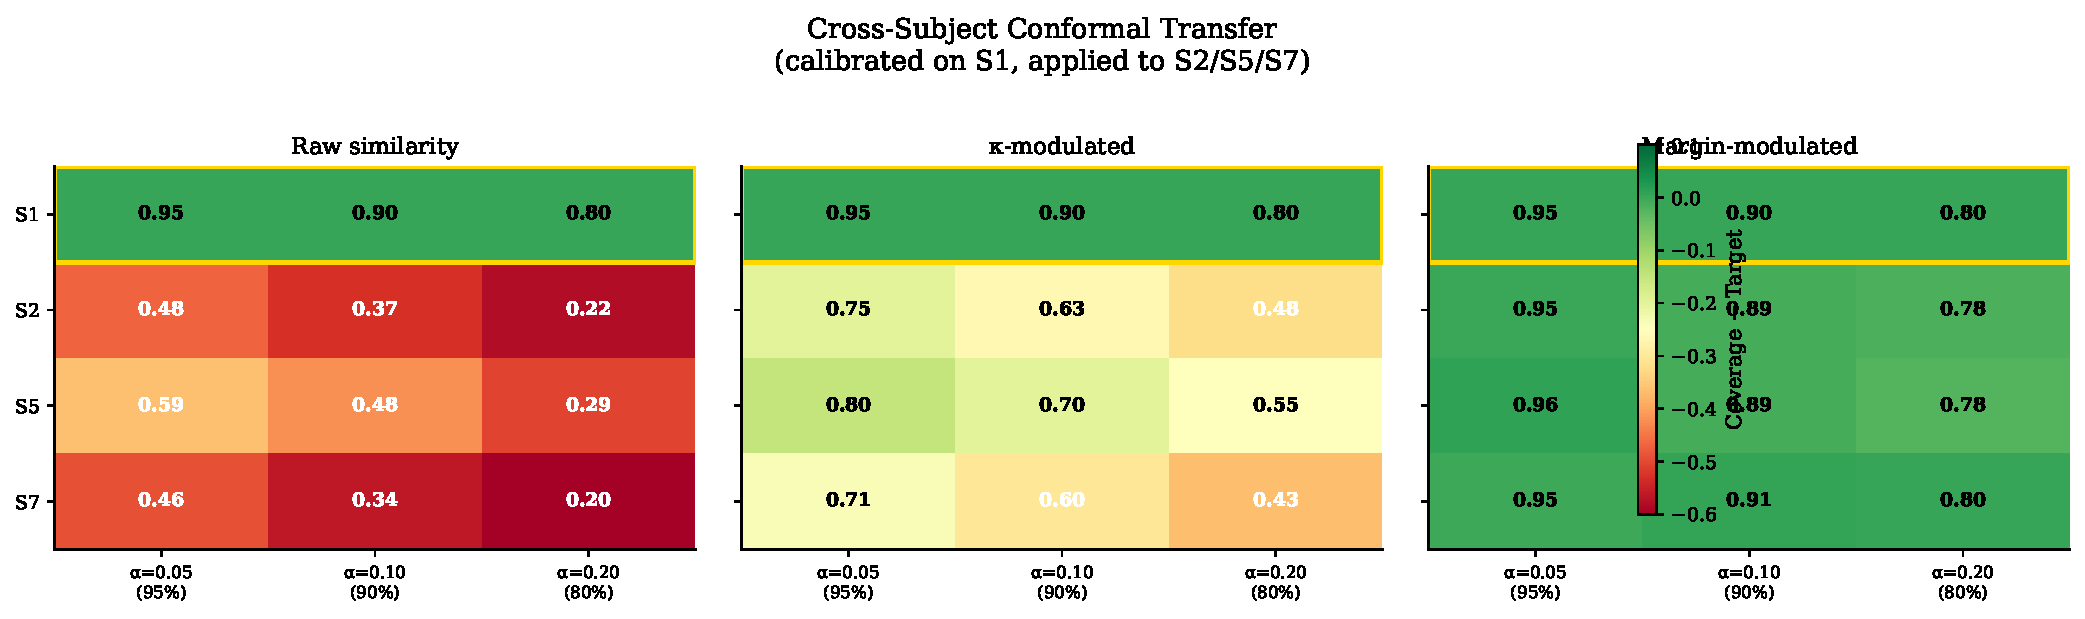
\includegraphics[width=\textwidth]{../figures/fig5_cross_subject_transfer.pdf}
    \caption{Cross-subject conformal transfer heatmap. Each cell shows empirical coverage when calibrated on S1 and applied to S2/S5/S7. Colors encode coverage $-$ target (green = valid, red = under-covered). \textbf{Margin-modulated scores (right) achieve near-perfect transfer}, while raw scores (left) fail catastrophically due to subject-specific similarity scales.}
    \label{fig:cross_subject}
\end{figure}

\paragraph{Why margin scores transfer.} Raw similarity scores are subject-specific: they depend on the decoder's absolute similarity scale ($\bar{\kappa}$ ranges from 13.5 to 28.8 across subjects). The $\kappa$-modulated score partially corrects by normalizing per-subject, but the $\kappa$ scales themselves differ. In contrast, the margin --- the gap between the top-1 and top-2 similarities --- captures \emph{relative discriminability} that is largely invariant to the absolute similarity scale. This produces nonconformity scores whose quantile structure is preserved across subjects.

\paragraph{Comparison to per-subject calibration.} Per-subject calibration (splitting each subject's data 50/50) achieves valid coverage for all subjects and scores (Table~\ref{tab:self_vs_cross}), confirming that the exchangeability assumption holds within each subject. The margin-modulated score is unique in that it achieves comparable performance \emph{without} per-subject calibration data.

\begin{table}[t]
\centering
\caption{Self-calibrated vs.\ cross-subject coverage (raw similarity, $\alpha=0.05$). Self-calibration always works; the coverage gap quantifies the distribution shift.}
\label{tab:self_vs_cross}
\begin{tabular}{lccc}
\toprule
Subject & Self-calibrated & Cross-subject & Gap \\
\midrule
S1 & 96.0\% & 95.2\% & 0.8\% \\
S2 & 97.4\% & 48.1\% & 49.3\% \\
S5 & 94.6\% & 58.7\% & 35.9\% \\
S7 & 96.0\% & 45.8\% & 50.2\% \\
\bottomrule
\end{tabular}
\end{table}

\section{Per-ROI Conformal Decomposition}
\label{sec:roi}

Using a Directional Consensus Fusion (DCF) decoder with 16 per-ROI vMF expert heads, we decompose confidence by brain region. Category-selective regions show significantly higher $\kappa$ for their preferred stimulus categories: PPA (places, Cohen's $d=0.73$), FFA1 (faces, $d=0.26$). The 16-dimensional $\kappa$ vector alone achieves 43.5\% category decoding accuracy across 12 COCO supercategories (chance $= 27.5\%$, $p < 0.001$), indicating that confidence patterns carry semantic information beyond mere image discriminability.

\begin{figure}[t]
    \centering
    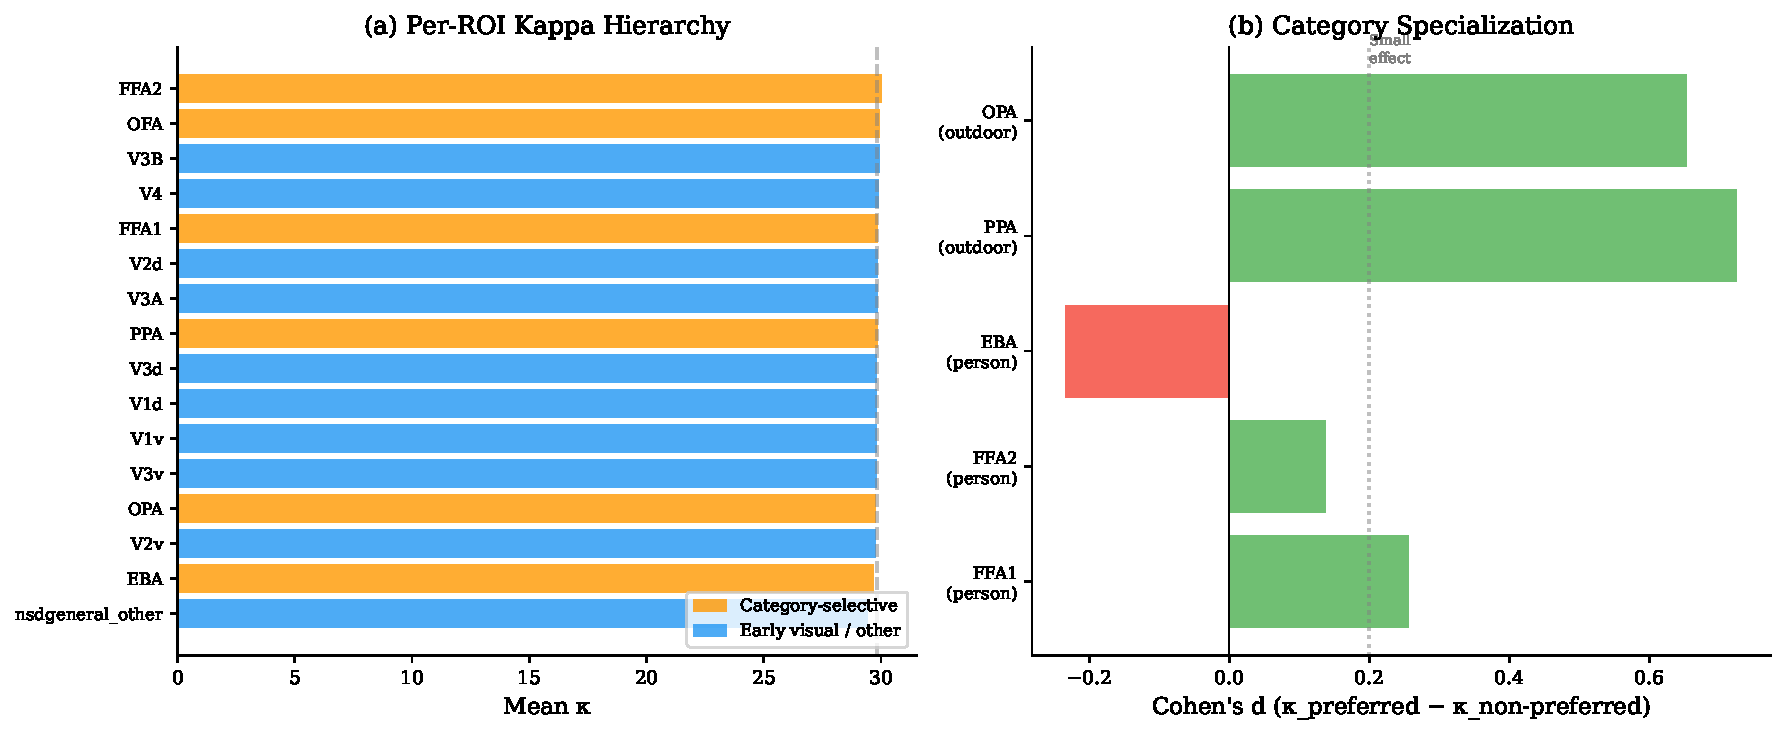
\includegraphics[width=\textwidth]{../figures/fig4_roi_specialization.pdf}
    \caption{(a) Per-ROI $\kappa$ hierarchy from the DCF decoder. Category-selective regions (orange) tend toward higher $\kappa$ than early visual areas (blue). (b) Category specialization effect sizes: PPA shows the strongest effect ($d=0.73$), consistent with its known place selectivity.}
    \label{fig:roi}
\end{figure}

\section{Discussion}

\paragraph{Practical implications for BCIs.} Our results establish three levels of reliability for neural decoding: (1)~Within-subject conformal prediction is straightforward and provides exact guarantees with modest calibration data ($n \approx 500$). (2)~Cross-subject transfer via margin-modulated scores opens the door to population-level BCI calibration, drastically reducing per-user setup time. (3)~The $\kappa$-stratified analysis provides an \emph{instance-level} confidence signal: high-$\kappa$ trials can be trusted; low-$\kappa$ trials should be flagged.

\paragraph{Limitations.} Our evaluation is limited to the retrieval setting ($m=1000$ gallery) rather than open-vocabulary generation. The cross-subject transfer, while promising, operates on subjects scanned with the same protocol. Session-level and scanner-level distributional shift remain open questions. Additionally, the margin-modulated score's cross-subject validity likely reflects the relatively homogeneous SHARED1000 stimulus set; more diverse stimuli may introduce covariate shift.

\paragraph{Broader impact.} While conformal prediction provides formal guarantees, it does not prevent misuse of decoded brain content. Ethical safeguards around consent and privacy remain essential.

\section{Conclusion}

We introduced the first framework for distribution-free reliability guarantees in neural image decoding. Three findings stand out: conformal prediction with vMF-tailored scores produces valid prediction sets across all coverage levels; the margin-modulated nonconformity score enables cross-subject transfer with $<3\%$ coverage gap; and the $\kappa$-stratified analysis reveals that the vMF concentration parameter captures genuine neural signal reliability. Together, these results establish conformal prediction as a practical and theoretically grounded tool for trustworthy brain-computer interfaces.

\bibliography{references}
\bibliographystyle{plainnat}

\end{document}
